\documentclass[../../main.tex]{subfiles}
\begin{document}
\section{Funzioni continue}
Una funzione $f$ è continua in un punto $x_0$ se:
\[
    \lim_{x\to x_0} f(x) = f(x_0)
\]
(cioè se il valore limite, per $x$ che tende a $x_0$, è uguale al valore della funzione in $x_0$).\\
Una funzione è continua in un intervallo $[a, b]$ se è continua in ogni punto $x_0 \in [a, b]$.
(se $x_0 = a$ si considera il limite destro, se $x_0 = b$ si considera il limite sinistro).\\
Abbiamo visto, ad esempio, che $\lim_{x\to 0} \sin x = 0 = \sin 0$ e $\lim_{x\to 0} \cos x = 1 = \cos 0$;
$\implies$ le funzioni $\sin x$ e $\cos x$ sono continue per $x=0$ ed anche per ogni altro $x_0 \in \mathbb{R}$.\\
Si dimostra anche che tutte le funzioni elementari sono continue. Potrei avere una discontinuità quando ho un denominatore come $f(x) = \dfrac{\sin x}{x}$
che non è definita in $x=0$.

\subsection{Punti di discontinuità}
I punti di discontinuità sono i punti in cui la funzione non è continua.
\subsubsection{Discontinuità eliminabile}
$x_0$ è il punto di \textbf{discontinuità eliminabile} se esiste il limite di $f$ in $x_0$ e risulta:
\[
    \lim_{x\to x_0} f(x) \neq f(x_0)
\]

\subsubsection{Discontinuità di prima specie}
$f(x)$ presenta in $x_0$ una \textbf{discontinuità di prima specie} se esistono finiti i limiti destro e sinistro di $f$ in $x_0$ e si ha:
\[
    \lim_{x\to x_0^+} f(x) \neq \lim_{x\to x_0^-} f(x)
\]

\subsubsection{Discontinuità di seconda specie}
$f(x)$ presenta in $x_0$ una \textbf{discontinuità di seconda specie} se almeno uno dei due limiti non esiste o è infinito.

\subsection{Teoremi sulle funzioni continue}
\subsubsection{Teorema della permanenza del segno}
Sia $f$ una funzione definita in un intorno di $x_0$ e sia continua in $x_0$
($\lim_{x\to x_0} f(x) = f(x_0)$).\\ Se $f(x_0) > 0$ allora esiste un numero
$\delta > 0$ con la proprietà che $f(x) > 0$ per ogni $x\in (x_0 - \delta, x_0
    + \delta)$.\\ \textbf{Dimostrazione:} la funzione è continua in $x_0$, cioè
$\lim_{x\to x_0} f(x) = f(x_0)$ quindi per definizione di limite:
\[
    \forall\varepsilon > 0, \ \exists\delta > 0 \ : \ \forall x, \ x\neq x_0, \ |x-x_0| < \delta \implies |f(x) - f(x_0)| < \varepsilon
\]
scelgo $\varepsilon = \dfrac{f(x_0)}{2}$, quindi:
\[
    |f(x) - f(x_0)| < \frac{f(x_0)}{2} \implies -\frac{f(x_0)}{2} < f(x) - f(x_0) < \frac{f(x_0)}{2}
\]
\[
    f(x) > f(x_0) - \frac{f(x_0)}{2} = \frac{f(x_0)}{2} > 0 \ \ \ \forall x\in (x_0 - \delta, x_0 + \delta)
\]
\textbf{Corollario:} Se $f(x)$ è continua in $x_0$ e $f(x)\geq 0$ o $f(x) > 0 \ \ \forall x\in (x_0 - \delta, x_0 + \delta)$ allora $f(x_0) \geq 0$.

\subsubsection{Teorema dell'esistenza degli zeri}
Sia $f(x)$ una funzione continua in un intervallo $[a, b]$. \\ Se $f(a) < 0$ e
$f(b) > 0$ allora esiste almeno un punto $x_0 \in (a, b)$ tale che $f(x_0) =
    0$.\\ \textbf{Dimostrazione:} troppo lunga guarda pagine 11-25 lez 06.

\subsubsection{Teorema dell'esistenza dei valori intermedi}
Una funzione continuia in un intervallo $[a, b]$ assume tutti valori compresi
tra $f(a)$ e $f(b)$. \textbf{Dimostrazione:} Consideriamo il caso in cui $f(a)
    \leq f(b)$.\\ Dobbiamo provare che $\forall y_0 \in [f(a), f(b)] \ \exists
    x_0\in[a, b]$ tale che $f(x_0) = y_0$.
\begin{itemize}
    \item Se $y_0 = f(a)$, possiamo prendere $x_0 = a$ e analogamente se $y_0 = f(b)$
          possiamo prendere $x_0 = b$.
    \item Se $y_0 \in (f(a), f(b))$, consideriamo la funzione:
\end{itemize}
\[
    g(x) = f(x) - y_0 \ \ \ \forall x\in [a, b]
\]
e calcolata in $x = a$ e $x = b$\\
\[
    g(a) = f(a) - y_0 \ \ \ \ g(b) = f(b) - y_0 \implies g(a) < 0 \ \ \ \ g(b) > 0
\]
Applicando quindi il teorema dell'esistenza degli zeri alla funzione $g(x)
    \implies$
\[
    \exists x_0\in(a,b) \ : \ g(x_0) = 0 \implies f(x_0) = y_0 \ \ \ \clubsuit
\]

\subsubsection{Teorema di Weierstrass}
Sia $f(x)$ una funzione continua in un intervallo chiuso e limitato $[a, b]$.
Allora $f(x)$ assume minimo e massimo in $[a, b]$.\\ Cioè esistono $x_1, x_2$
in $[a, b]$ che sono detti rispettivamente punti di minomo e di massimo per
$f(x)$ nell'intervallo $[a, b]$.\\ I corrispondenti valori $m = f(x_1)$ e $M =
    f(x_2)$ sono detti \textbf{minimo} e \textbf{massimo} di $f(x)$ in $[a, b]$.
\begin{center}
    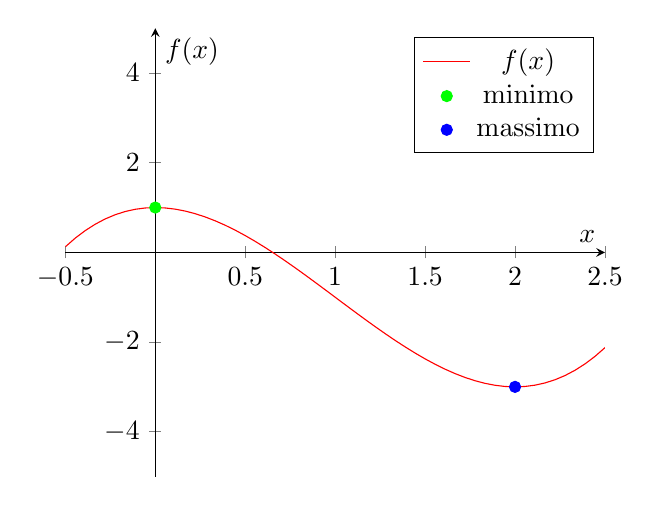
\begin{tikzpicture}
        \begin{axis}[
                axis lines = center,
                xlabel = $x$,
                ylabel = {$f(x)$},
                xmin = -0.5,
                xmax = 2.5,
                ymin = -5,
                ymax = 5,
            ]
            \addplot [
                domain=-0.5:5,
                samples=100,
                color=red,
            ]
            {x^3 - 3*x^2 + 1};
            \addlegendentry{$f(x)$}

            \addplot [only marks, mark = *, color=green] coordinates {(0, 1)};
            \addlegendentry{minimo}

            \addplot [only marks, mark = *, color=blue] coordinates {(2, -3)};
            \addlegendentry{massimo}
        \end{axis}
    \end{tikzpicture}
\end{center}
\textbf{Dimostrazione:} Hp: funzione continua in un intervallo chiuso e limitato.\\
Poniamo $M = \sup \{f(x) : x\in [a, b]\}$ esiste, potrebbe essere $M < +\infty$ o $M = +\infty$. \\
Verifichiamo ora che $\exists x_n\in[a, b] \ : \ \lim_{n\to+\infty} f(x_n) = M (\star)$.
\begin{itemize}
    \item Se $M = +\infty$, per le proprietà dell'estremo superiore, $\forall n\in
              \mathbb{N}, \exists x_n\in[a, b] \ : \ f(x_n) > n$. Per il teorema di confronto
          $f(x_n) \to M = +\infty$.
    \item Se invece $M < +\infty$, sempre per le proprietà dell'estremo superiore,
          $\forall n\in \mathbb{N}, \ \exists x_n\in[a,b]$ tale che \\ $M - \dfrac{1}{n}
              < f(x_n) \leq M$ e quindi $f(x_n) \to M$ per il teorema dei carabinieri.
          $(\star) \ \ \lim_{m\to+\infty} f(x_n) = M$
    \item Per il teorema di Bolzano-Weierstrass, da $x_n \subset [a, b] \text{
                  (limitate)}$, esiste una estratta $x_{nk}$ convergente ad un punto $x_0\in[a,
                  b]$.
          \[
              x_{nk} \to x_0
          \]
          Ma poichè la funzione è continua:
          \[
              f(x_{nk}) \to f(x_0) \ \ \ (n \to +\infty)
          \]
          Allora
          \[
              M = \lim_{n\to+\infty} f(x_n) = \lim_{k\to+\infty} f(x_{nk}) = f(x_0) \implies M = f(x_0)
          \]
          Quindi abbiamo dimostrato che $M$ è un massimo perchè:
          \[
              f(x_0) = M = \sup \{f(x) : x\in[a, b]\} \text{ è un massimo} \ \ \clubsuit
          \]
\end{itemize}
\textbf{Conseguenza:} La funzione è limitata, dal massimo e minimo.\\

Possiamo ora dare una nuova formulazione del teorema di esistenza dei valori
intermedi.

\subsubsection{Teorema di esistenza dei valori intermedi (formulazione II)}
Una funzione continua in un intervallo $[a,b]$ ammette tutti i valori compresi
tra il massimo e il minimo. Tra i risultati sulle funzioni continue, si
dimostra come applicazione, anche il seguente:
\subsubsection{Criterio di invertibilità}
Una funzione continua e stretteamente monotona in un intervallo $[a ,b]$ è
invertibile in tale intervallo.

\end{document}